\newpage
\section{Context: Hydrocarbon Exploration}

The processes of creating images of the underground is primarily used in the field of hydrocarbon exploration. This relatively recent field has its origins in the 1900's, but most of the major oil pockets have already been discovered and now the job of hydrocarbon exploration becomes more difficult and necessary in underground zones that are smaller and harder to image. Add to this the difficulties of the often mountainous or forest-heavy terrain above the surface, and we can see that the hydrocarbon exploration is an increasingly complicated field in both the geophysical and mathematical domains. 

The cost of discovering a barrel has skyrocketed more than three-fold over the last decade due to these increasingly inhospitable environmental conditions and a fairly constant reduction of existing reserves at $5-15\%$ per year \cite{hydrocarbonExplorationCosts}. In addition, political risks associated with the discovery and drilling of new oil wells have been escalating. For example, the USA, Russia, Canada, Denmark, Iceland, and Norway have competing claims over the Arctic Circle where approximately a fifth of the world's recoverable oil is contained. Although Uganda has more than 2 billion barrels of oil, necessary negotiations between the government and oil companies have been slow. In 2009, 3D seismic surveys cost on average between \$40,000 and \$100,000 per square mile. \cite{hydrocarbonExplorationCosts}

In the domain of hydrocarbon exploration, there is a long and complicated sequence of data processing given the seismic surveys generated from the energy sources and receivers. The goal of this sequence of steps is to generate from the data an accurate image of the 3-dimensional interior of the earth for analysis by geophysicists. Specifically, the data consists of the measurement of energy that the receivers record over time after a signal has been sent by the source and reflected by heterogeneities within the earth.

\subsection{Seismic Acquisition}

\begin{figure}[ht]
	\centering
	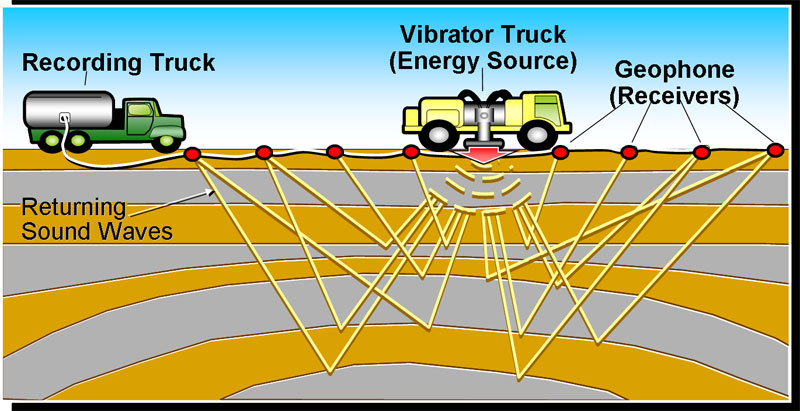
\includegraphics[width=0.39\textheight]{Images/SeismicChes5.jpg}
	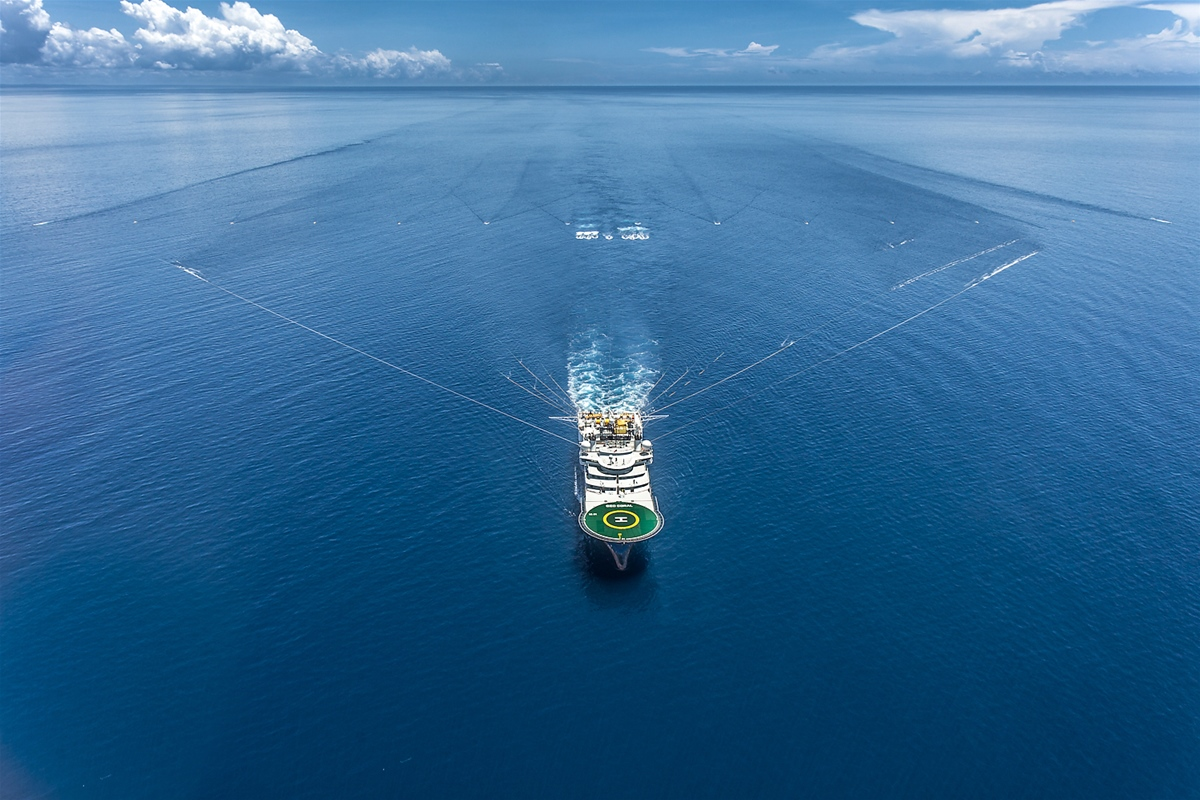
\includegraphics[width=0.3\textheight]{Images/2562_geo_coral_large.jpg}
	\caption{Model of Source and Receivers in land and maritime environments}
	\label{fig:Seismic-Acquisition}
\end{figure}

Seismic acquisition is the process of gathering the data, sometimes called seismic surveys, from the receivers, whether it be in a land or maritime environment. Typically, it involves one source, which can be a vibroseis / vibrator truck or dynamite, that sends out a pulse or multiple pulses also known as seismic waves. Due to differences in physical characteristics in the underground media, the signal may get refracted, reflected, or converted. 

\begin{figure}[ht]
	\centering
	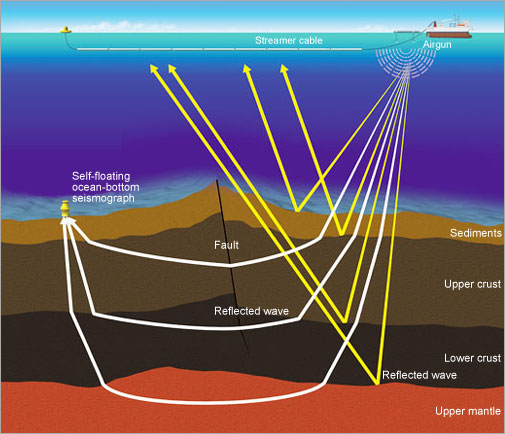
\includegraphics[width=0.7\textwidth]{Images/seabed_img_01.jpg}
	\caption{Hypothetical reflected and refracted waves used to model the seabed}
	\label{fig:Rays-Reflection-And-Refraction}
\end{figure}

\begin{enumerate}
	\item
	\textbf{Reflection}: When the wave encounters a change in \textbf{acoustic impedance} (propagation velocity multiplied by density of the medium), part of the energy of the wave is reflected in the direction from which it came. The fraction of energy that is reflected is called the \textbf{reflection coefficient}. in certain media that are called \textbf{anisotropic}, it depends on the incidence angle. Otherwise the media are called \textbf{isotropic}.
	\item
	\textbf{Refraction}: When the wave encounters a difference in \textbf{propagation velocity}, the wave refracts and changes its direction according to Snell's law. 
\end{enumerate}

Both of these resulting waves are used respectively in seismic reflection and seismic refraction techniques, although seismic reflection is more often used. See Figure ~\ref{fig:Rays-Reflection-And-Refraction} for the ray model and Figure ~\ref{fig:Wavefield-Reflection-And-Refraction} for the wavefield model in a simulated environment.

\begin{figure}[ht]
	\centering
	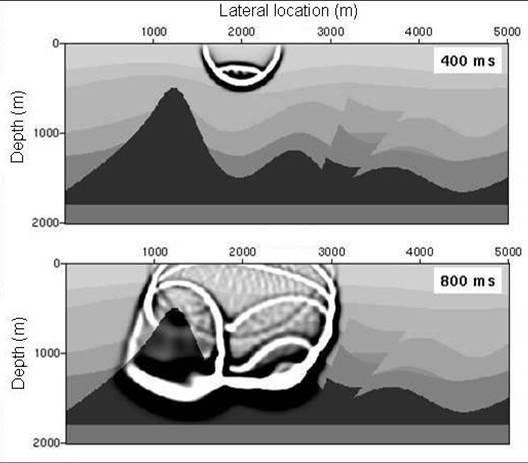
\includegraphics[width=0.7\textwidth]{Images/reflectionrefraction.jpg}
	\caption{Simulated wavefield shown reflecting and refracting across different media}
	\label{fig:Wavefield-Reflection-And-Refraction}
\end{figure}

\subsection{Seismic Processing}

Seismic imaging, the steps required to create an image, is only one of the final parts of the entire process called seismic processing, the processing of the data obtained at the receivers. The whole course of seismic processing includes the pre-processing, which "addresses topics such as source signature processing, noise elimination, static corrections, or multiple removals" as well as removing the effects of multiple reflections in classical seismic imaging techniques \cite{EAGE}.

\subsection{Seismic Waves}

Seismic waves are essentially movement of the earth that may be caused artificially by a thumper truck, seismic vibrator, or dynamite or may be caused naturally by an earthquake or sudden breaking of a rock. There exist two main types of seismic waves: body waves and surface waves. As the name suggests, surface waves travel at the surface of the earth, similarly to water ripples. Body waves travel in the interior of the earth, and like sound waves, can be either longitudinal or transverse waves most commonly referred to as P and S waves.

\subsubsection{Body Waves}

\begin{enumerate}[leftmargin=0.5in]
	\item{\textbf{P Waves}} is short for Primary Waves or Pressure Waves. As a longitudinal wave, they cause the earth to compress and rarefy in the same direction as the wave movement. In other words, they cause the pressure of the earth to oscillate. Other examples include sound waves and stretched slinky toys. These waves propagate more quickly than S Waves.
	
	\item{\textbf{S Waves}} is short for Secondary Waves or Shear Waves. Moving more slowly than the P Waves, they cause the earth to move up and down perpendicular to the wave movement.
\end{enumerate}

\begin{figure}[ht]
	\centering
	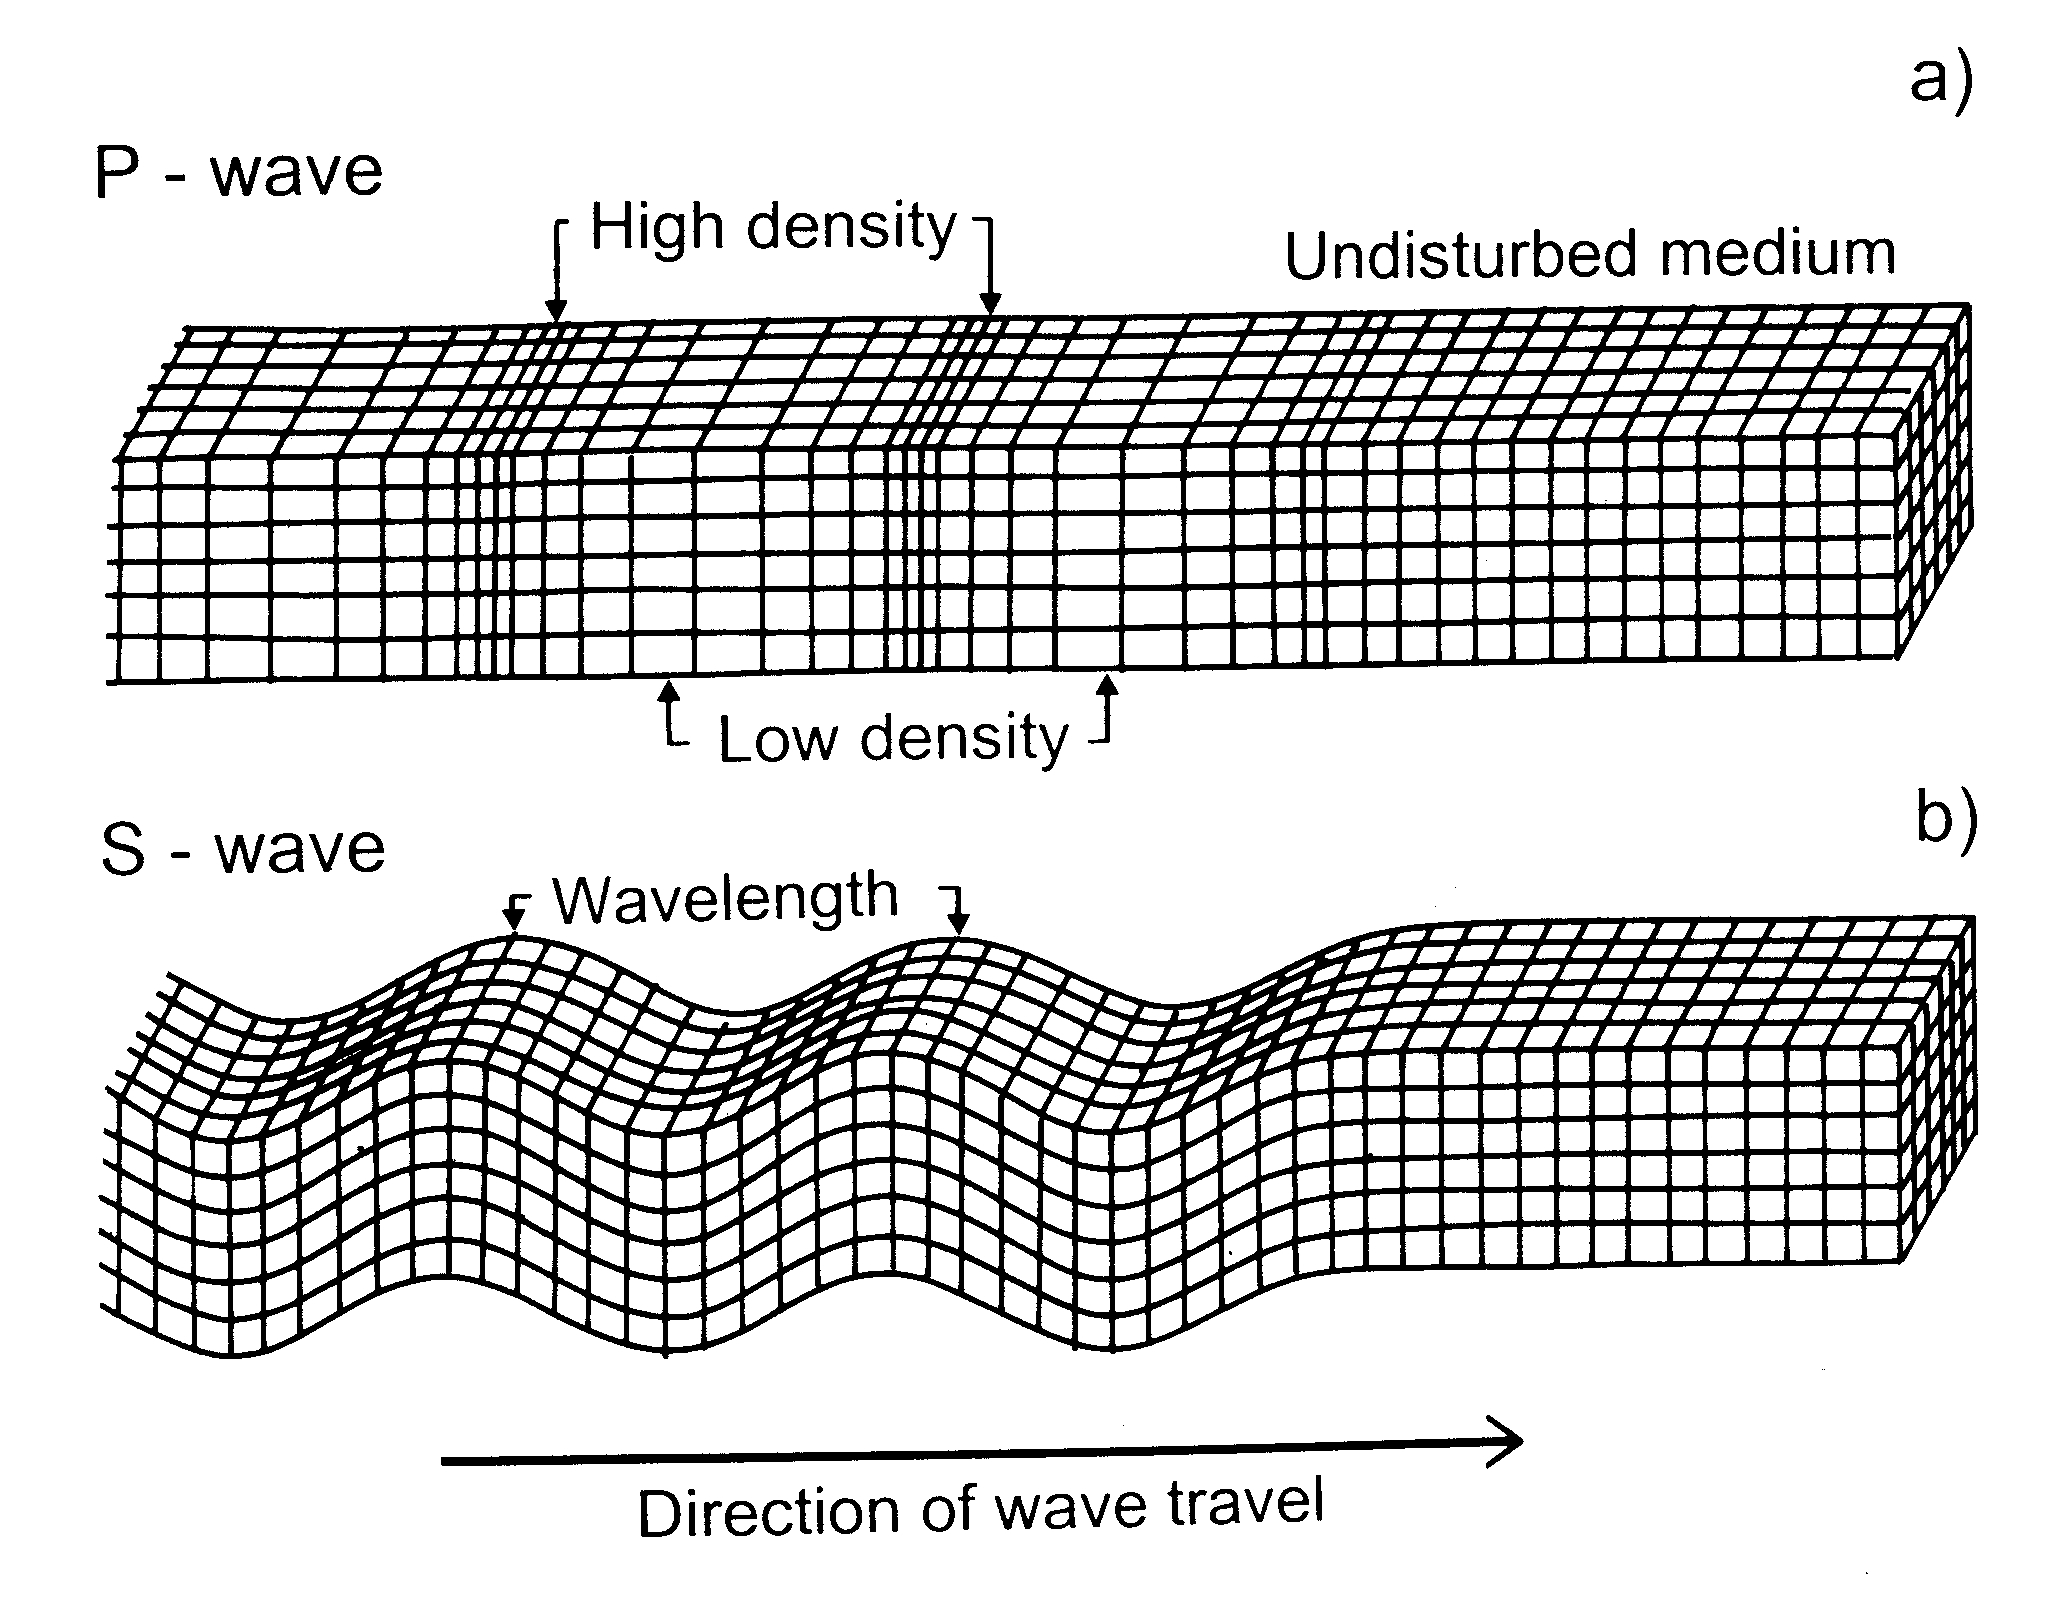
\includegraphics[width=0.7\textwidth]{Images/waves.jpg}
	\caption{P and S Waves}
	\label{fig:PSWaves}
\end{figure}

\subsubsection{Surface Waves}

There are several different types of surface waves, including Rayleigh and Love types. Because they propagate along the surface in two dimensions instead of in three dimensions like body waves, their amplitude tend to dissipate less quickly and they tend to cause more damage. Examples of waves that may be classified as surface waves include waves that travel at the interface between elastic and acoustic (ground and water) environments, as well as ripple-like waves at the very surface.

\begin{figure}[ht]
	\centering
	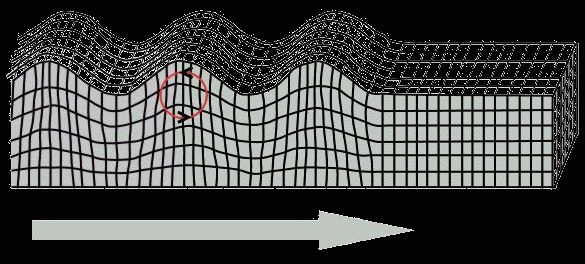
\includegraphics[width=0.7\textwidth]{Images/Rayleigh_surface_waves.jpg}
	\caption{Rayleigh Surface Wave}
	\label{fig:SurfaceWaves}
\end{figure}























